\documentclass[11pt,a4paper]{scrartcl}
\typearea{12}
\usepackage{graphicx}
\usepackage{pstricks}
\usepackage{listings}
\lstset{language=python}
\pagestyle{headings}
\newcommand{\turtle}{\texttt{Turtle}\,}
\newcommand{\lnn}[1]{\textbf{line #1}\,}
\newcommand{\Lnn}[1]{\textbf{Line #1}\,}
\markright{Python turtle worksheet}
\begin{document}
\subsection*{Introduction}
Here is a simple turtle programme (\texttt{turtle\_doing\_nothing.py}):
\begin{lstlisting}[numbers=left]
from turtle import *

tom=Turtle()

tom.getscreen()._root.mainloop()
\end{lstlisting}
\Lnn{1} and \lnn{5} aren't worth spending much time on at first, the first
line imports the library of commands related to turtle, \lnn{5}
prevents the computer from closing the graphics window when the
programme has finished running; we won't include this line again,
though it is needed. \Lnn{3} is important, it tells the computer to
make an object, in this case a \turtle and call it \texttt{tom}, it
knows what a \turtle is from the library it imported in line 1; in the
instructions on what to do when making a \turtle the computer is told
to open a graphics window and to draw the turtle, a little arrow
shape.
\begin{center}
\fbox{

\includegraphics[width=10cm]{code/turtle_doing_nothing.eps}}
\end{center}

Here the turtle does something (\texttt{line.py}):
\begin{lstlisting}[numbers=left]
from turtle import *

tom=Turtle()

tom.forward(100)
\end{lstlisting}
The extra line, \lnn{5}, tells the turtle to move forward by 100 units,
this is an important piece of Python syntax, to tell an object to do
something you use a dot followed by the command, here it tells the
\turtle called \texttt{tom} to perform the command
\texttt{forward}. Of course, the command has to make sense for
whatever type of object it is dotted onto, but here it does,
\texttt{forward} is one of the defined commands for a \turtle object.
\begin{center}
\fbox{
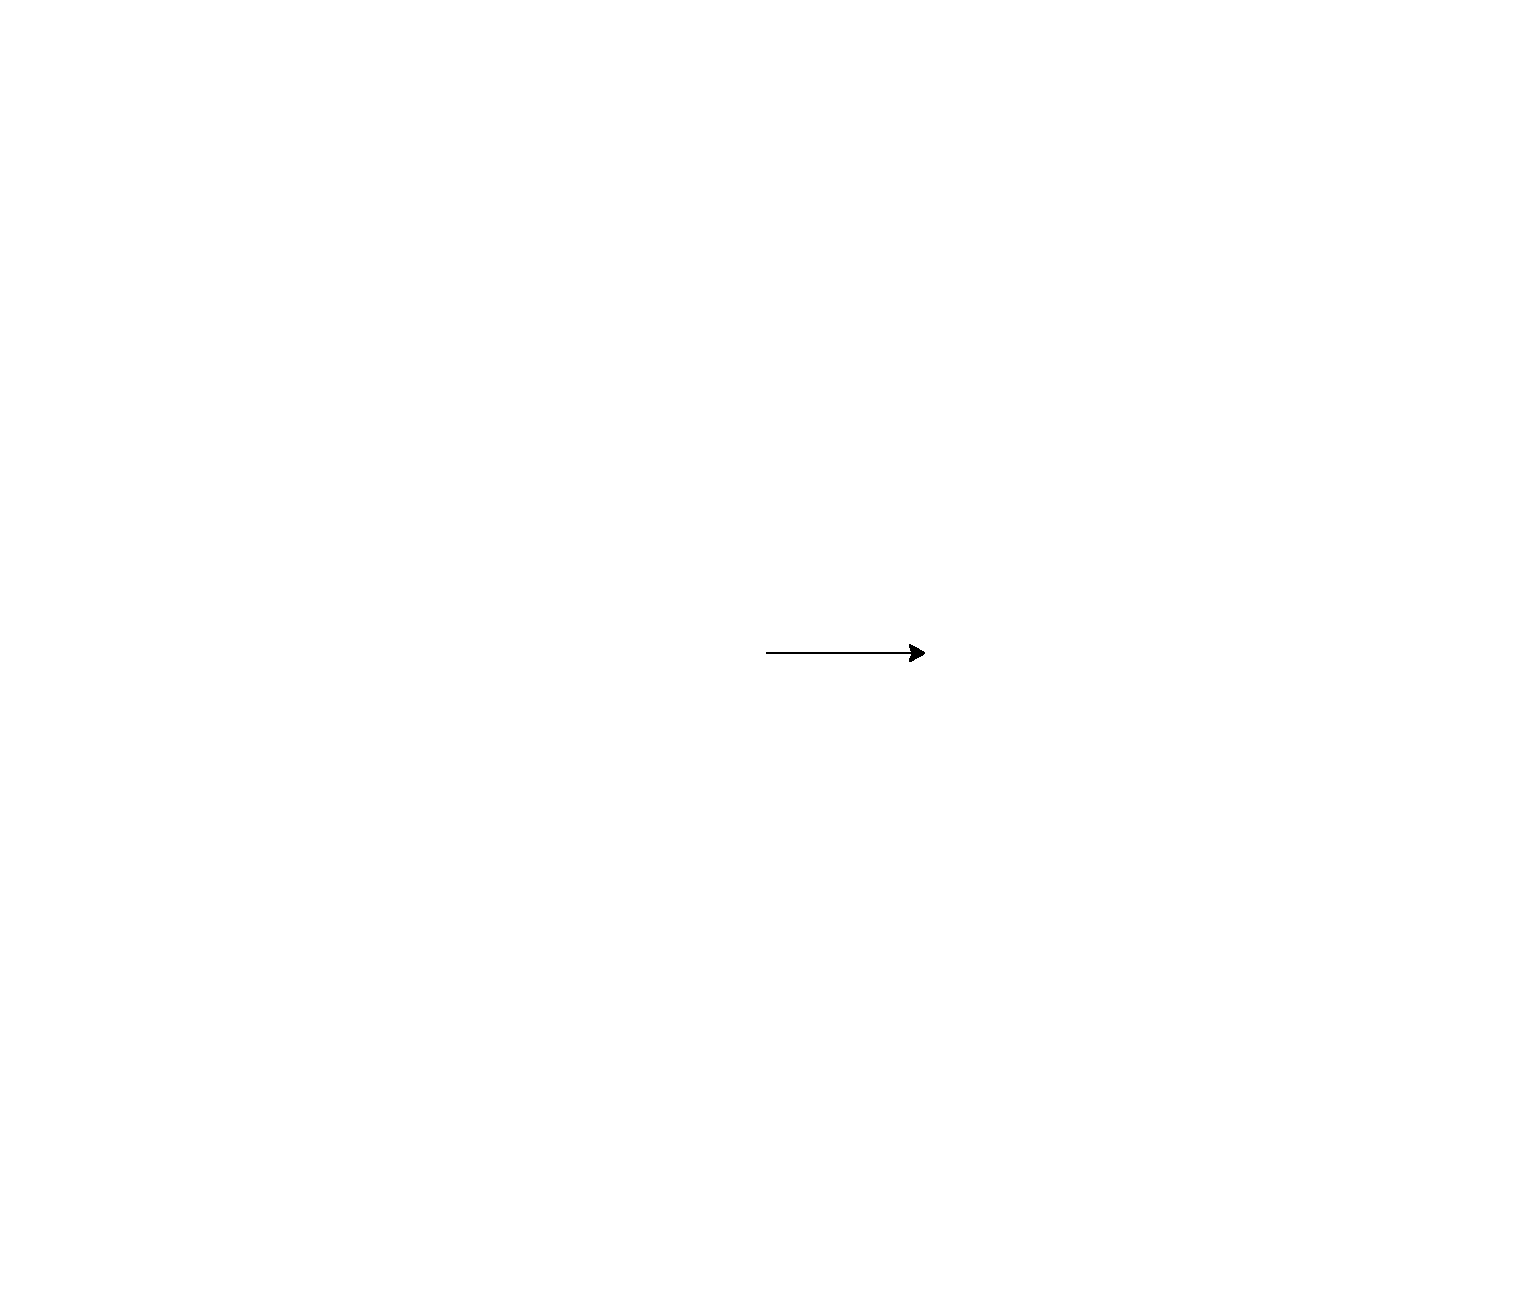
\includegraphics[width=10cm]{code/line.eps}}
\end{center}

\turtle objects have another command \texttt{right(90)} which turns the turtle by $90^\circ$. Can you write a programme to draw this:
\begin{center}
\fbox{
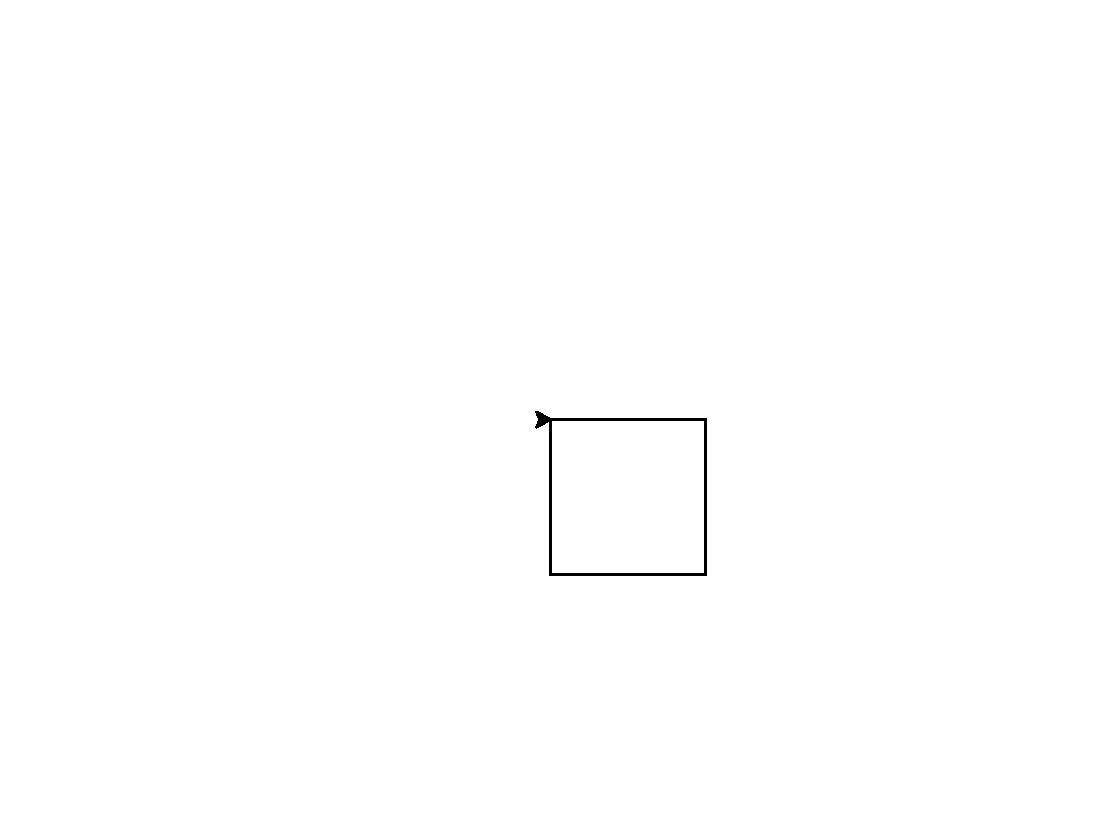
\includegraphics[width=10cm]{code/right_angle.eps}}
\end{center}
How about a square?
\begin{center}
\fbox{
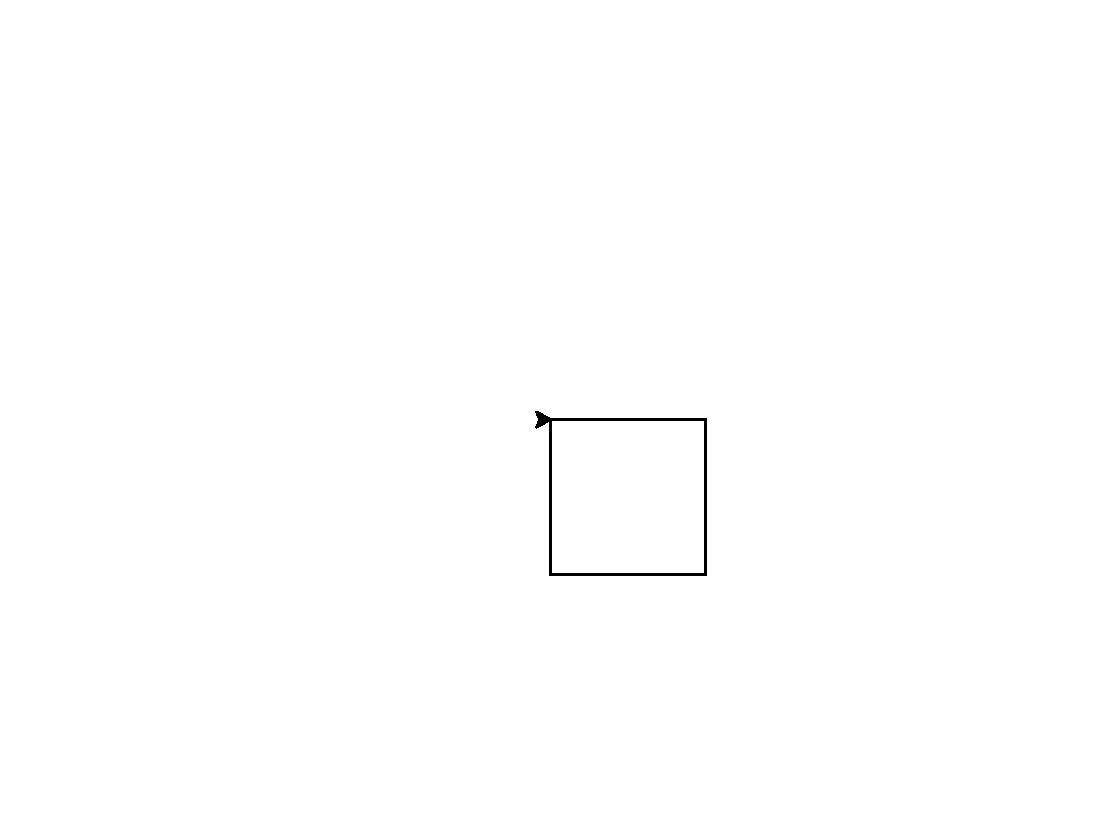
\includegraphics[width=10cm]{code/square.eps}}
\end{center}

\end{document}

